\documentclass[pdftex,a4paper,14pt,english]{extarticle}

\usepackage[top=2cm,bottom=27mm,left=3cm,right=18mm]{geometry}
\usepackage[utf8]{inputenc}
\usepackage[english]{babel}
\usepackage[pdftex]{hyperref}
\usepackage{indentfirst}
\usepackage[pdftex]{graphicx}
\usepackage{amsmath}
\usepackage{amssymb}
\usepackage{ragged2e}
\usepackage{multirow}
\usepackage{algorithmic
}\usepackage[boxed]{algorithm}
\usepackage{tabularx}
\usepackage{xtab}
\usepackage{subfig}
\usepackage{hyphenat}
\usepackage{setspace}
\usepackage{fancyhdr}
\usepackage{tikz}

\usetikzlibrary{positioning,fit,calc}

\pgfkeys{
    /tikz/node distance/.append code={
        \pgfkeyssetvalue{/tikz/node distance value}{#1}
    }
}

\pagestyle{fancyplain}
\fancyhf{}
\renewcommand{\headrulewidth}{0pt}
\rfoot{\fancyplain{}{\thepage}}

\linespread{1.15}
\floatname{algorithm}{Algorithm}

\addto\captionsrussian{\renewcommand{\contentsname}{Content}}

% new commands
\newcommand\sign[1]{sign(#1)}

\begin{document}

\setcounter{page}{1}
\tableofcontents
\newpage

\section{Introduction}
\addcontentsline{toc}{section}{Introduction}

\subsection{Background}

The thesis project is done in the company \textit{Accedo Broadband AB}. \textit{Accedo is the market leading enabler of TV application solutions. Accedo provides applications, tools and services to media companies, consumer electronics and TV operators globally, to help them deliver the next-generation TV experience. Accedo’s cloud-based platform solutions enable customers to cost-efficiently roll out and manage application offerings and stores for multiple devices and markets} \cite{Accedo}.

The main business of the company is developing smart user applications for customer APIs. Unfortunately, every customer API was developed in a unique way and has their own communication protocol. Consequently, it is difficult to write smart user applications that use many customer APIs because a developer would have to write the communication layer for every customer API. 

The problem can be defined as follows:  There are a lot applications written for different operating systems and they require frequent communication with many customer APIs. What architecture is the most appropriate for communication between applications and external services represented by a customer APIs? 

One of the solutions, is a simple direct communication between client and services. The client will send requests to every service and wait for responses. This solution has several drawbacks: a developer would have to maintain many communication layers written in different languages. When the external API changes, the developer would be forced to rewrite every communication layer. This increases the cost of development and the development time. Another problem is security, some services might have a private API that should not be used directly.

A different solution will be to introduce the middle layer between the client and external services. The client will communicate with middle layer using predefined protocol, middle layer will then gather data from external services and send it to the client. This approach has several benefits: every application will be written with standardised communication API, defined by the middle layer; if external API changes, only middle layer should be rewritten; the response time can be decreased by caching the data in the middle layer. 

Another solution can be the usage of CDN (Content Delivery Networks). The application will send the requests directly to the external services, but the request will be intercepted and handled by the CDN Edge Servers that are located between Application and External Services. This solution requires dynamic usage of HTTP Cache-Control headers. The advantage of using CDN is that the developer need not maintain the middleware service. Alternatively, the results will be cached somewhere on the way between Application and External services producing a faster response to the final user. On the other hand, the drawbacks are that it is difficult to configure CDN to process dynamic content and the developer would need to write the communication layer for every external service. 

This project tries to break the connection between applications and external services by providing the middle layer. The applications communicates with the middleware using a predefined format that is the same for every platform. The middleware will manage the requests, translate them to the format appropriate for the external services and forward them to the appropriate servers. It will also manage the responses from servers and send them back to the applications.


\subsection{Project Objectives}

The project is in the context of networking, caching and data aggregation. The goal of the project is to investigate different solutions for implementing a caching layer used in a backend middleware, design and develop prototypes for each solution, run set of tests and select the most optimal solution.
The selected solution is then further developed and integrated into an existing middleware provided by the company, and an analysis is then made in a real life scenario.


\subsection{Thesis Outline}

During the project the middleware server developed by company will be examined. The application will be studied and analysed in development environment. The set of problems and future improvements will be retrieved and discussed. The appropriate solutions for selected problems will be presented in this paper.

The Theory section will give the information about the modern web caching technologies and how they can be used on practice. Also, some parts of HTTP protocol will be introduced.

The Architecture overview will present the company solution and will identify the drawbacks. The web caching solution for some problems described in architecture overview will be introduced.

The HVG chapter will present the second part of the thesis: Hierarchical VMO Generator.

The Test chapter will compare the performance of Redis cache and Web cache solutions and evaluate the HVG algorithm in comparison with existing solution.

\newpage

%TODO investigate the code repositories
%TODO define the common pattern for the server interaction
%TODO define request/response types(what can be combined, what cannot) for client part
%TODO update the report, add information about types to the server achitecture, introduce new problem if exists 
%TODO Make dependencies to the json tree*
%TODO update report with the algorithm of request aggregation 
%TODO integrate json tree* to the VIA app
%TODO update the report, add information about integration
%TODO set the web cache with for the dynamic and static content between via and clients
%TODO set the web cache between via and ovp
\section{Theory}
	
\subsection{Content Delivery Networks}


Nowadays the Internet is available almost from any place in the world. It allows people from different countries to communicate with each other and exchange information. The content providers and applications should serve the user's requests from all around the world with the equally high speed in order to provide good user experience. For solving this task, companies should deploy their servers all around the world in multiple data centers. For world-class companies like Google and Netflix this task is solvable\cite{NetflixCDN}, but for middle sized companies there should be another solution because it is very expensive and sometimes complicated to deploy servers in multiple data centers. Fortunately, the content delivery networks solve this problem\cite{AkamaiCDN}.

The Content Delivery Network(CDN) is a distributed system consisted of many servers deployed all around the world in different data centers. They act as a local content holders. The routes to the content providers and applications are configured to lay through the CDN's servers. When the client wants to access the server through the Internet the request will be processed by the local CDN server and if it will find the data locally, it will deliver the response to the client without making the request to the content provider that can be located in different country. The CDNs can store both static and dynamic content. One of the first global solutions was presented by Akamai company\cite{AkamaiCDN}. The graphical architecture is depicted on figure \ref{fig:cdn_overview}.

The CDN consists of several parts: routing, load balancing and web caching\cite{CDNOverview}. The web caching part will be reviewed because it is relevant to the project.

\begin{figure}[h]
    \centering
    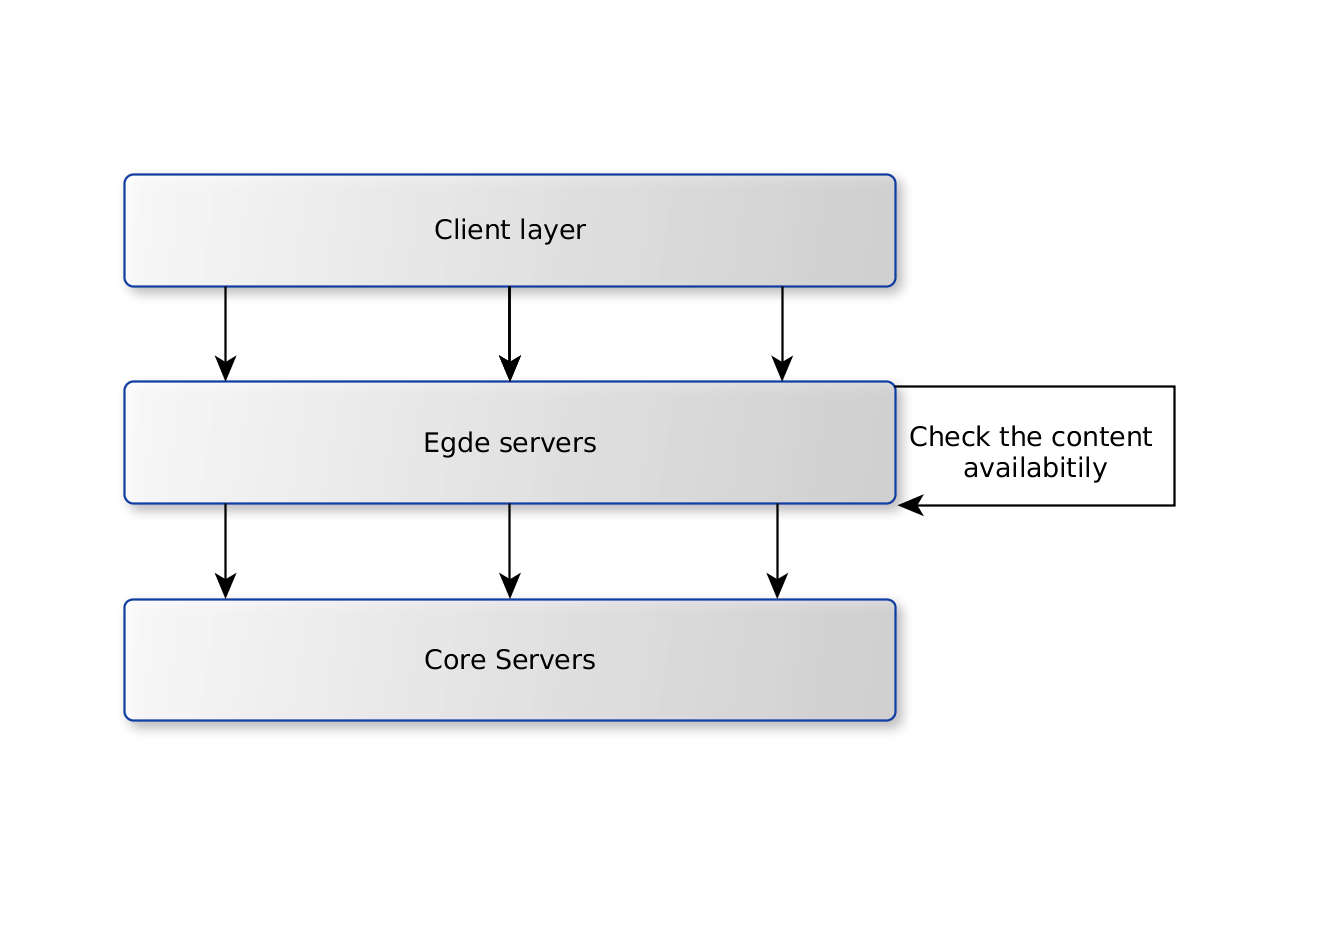
\includegraphics[width=\textwidth]{images/cdn_arch.png}
    \caption{Content Delivery Network Overview}
    \label{fig:cdn_overview}
\end{figure}

\subsection{Web Caching}

Web caching is the technique that allows to store temporary content that is requested from the Internet e.g. HTML pages, JSON, XML or CSS files. It alleviates the server's work by reducing the amount of requests to it and reduces bandwidth usage\cite{WebCachingInterior}. A web cache system serves as a communication point between client and sevrer. The client's requests and server's responses are routed through it. The web cache stores responses from the server and returns them without hitting the underlying server. It also can manipulate the request/response headers.

The benefits of web caching:

\begin{itemize}
    \item Reduces the server workload. Using web caching the requests will go through the cache and will touch server only if the data does not present in caches or the data is stale. That will reduce the amount of requests made to server.
    \item Web caching improves user experience. The data will be delivered faster to the end users.
    \item Reduces bandwidth
\end{itemize}

\subsubsection{Content types}

% Describe static and dynamic content types

The content stored by web caches can be static or dynamic.

The static content is a set of resources that stay the same no matter what was the user input. Static objects are identified by the unique path and can be cached for a long time by the web caches.

The dynamic content is generated at run-time, based on the user input\cite{DynamicWebCaching}. The dynamic requests almost always processed by severs. They are the main consumers of the web server's resources. The dynamic requests are time dependant meaning that in different time the same request can produce different output, as a result they cannot be cached for a long time by the web caches. Moreover, for security reasons, usually dynamic objects that contain client's personal data and preferences are configured in order not to be cached by the external web caches and CDNs.

However almost all dynamic content is static for a short period of time. It changes only when the internal resouces e.g. databases are altered. This gives a possibility to configure web cache for storing dynamic objects.

\subsubsection{Http Cache Control Headers}

Web cache is controlled by the http cache control headers\cite{RFC7234}. The control mechanisms can be specified on both request and response sides. There are several http headers that are relevant for the project: 
\begin{itemize}
    \item Cache-Control
    \item Vary header
    \item Etag, If-None-Match
    \item Last-Modified, If-Modified-Since
    \item Expires( for http 1.0 )
    \item Widely used extension headers, like X-Cache.
\end{itemize}

There are two caching techniques: Time based caching and Data based caching.

The time based caching is represented by the next http headers: \textit{Last-Modified} and \textit{If-Modified-Since}, \textit{Cache-Control} with \textit{s-maxage} parameter and \textit{Expires} header. Client sends the request with specified \textit{If-Modified-Since} header, where he indicates as a parameter the time when the content was modified. The server will check the type of the content which was requested and send the corresponding response. If the static content was requested, the server will check if the resource was changed since the date specified by the client in \textit{If-Modified-Since} header, and will send the new content with the code 200 and updated \textit{Last-Modified} header if it was modified, otherwise it will reply with the code 304(resouce not modified) without content and with old \textit{Last-Modified} header. The server usually does not set the Last-Modified header to the dynamic resources because it is hard to know where exactly they were modified. 
During the response the server can specify the \textit{Cache-Control} header with s-maxage parameter. In this case, if the content is public, it can be cached by the web cache servers for s-maxage time specified in seconds. If the next request will occur in the next \textit{s-maxage} seconds, the content will be served from the web cache. This technique is used for caching both dynamic and static content. The difference between static and dynamic content is that the s-maxage parameter fot the dynamic content is set dynamically, and it is static for the static content.(change the last sentence)

The data based caching is represented by the \textit{Etag} and \textit{If-None-Match} headers. It is supported since in HTTP/1.1. On the first request the server will compute the hash of the content and send it to the client in the Etag header. The client will remember the hash value in the \textit{If-None-Match} header. When the next request occurs, the server will recompute the hash of the content and will compare it with the value specified in the If-None-Math parameter. If the values are the same, the server will reply with the 304 code, without content and with the old Etag header, otherwise it will change the Etag header to the new value and send the normal response. 


The web cache can be implemented on: 

\begin{itemize}
    \item Client side, by using browser caches
    \item Proxy servers, by introducing the middle caching server between client and server.
    \item Server side, by implementing cache programmatically
\end{itemize}

Currently, the middleware server supports the server side caching with Redis in memory data store. We will introduce the proxy server caching and will see if it will give the benefit to the architecture.(move to abstract) 

\subsubsection{An overview of proxy server types}

A proxy server is a server that is deployed between client and server. It serves as a middle point in communication between clients and servers. The proxy server redirects requests to servers and responses from servres. It can improve the performance of the servers by storing the copies of frequently used resources. When a client makes a request to the server through the proxy server, the  proxy server serves as a web cache, it will try to find data locally and will return the resource back to the client on success.

There are two main types of proxy servers: forward and reversed proxy\cite{WWWCaching}.
A forward proxy is a one of the most common types of proxy servers. The client is aware about the proxy server and can configure requests through it.
A reversed proxy is deployed by server administrators in the internal network. The client contacts the desired server, but the request is routed through the reversed proxy server. In this case, the client may not know about the underlying proxy. 
The reversed proxy server was selected for the project because it perfectly suits the architecture, the client should not know about the existence of the middle point. (and the web caching is mostly done by using reversed proxy servers).


\subsection{Http Session Management}

HTTP protocol is stateless by its nature, meaning that there is no possibility to distinguish one request from another. Http requests usually open new connection to the desired server every time. Nowadays, server can specify \textit{Keep-Alive} header in the response in order to give browser a hint that this connection can be used again for the new request. Unfortunately, without transferring user-specific information it is impossible to distinguish users.  

The session management is implemented through header fields  \textit{Set-Cookie} and \textit{Cookie} headers. When server wants to distinguish one user from another it sets the unique identifies for the user. This identifier is transferred in the header field Set-Cookie. The browser will parse this field and remember the unique identifier. For every new request, browser will send this identifier it header field Cookie. Of course server can send additional information in Set-Cookie header, that is unique for user. Unfortunately, it is very dangerous to transfer private information(e.g. credit card number) this way. The server can store dictionary of user ids and corresponding private information in memory and retrieve this information every time when the browser specifies Cookie header. 


\newpage



\section{Architecture Web}

\subsection{HTTP Protocol}

\subsection{SPDY Protocol}

\subsection{Web Caching Architecture}

\newpage

\section{Middleware Architecture}

\subsection{Server Architecture}

The company architecture contains the following components: Client Application, Middleware server, Middleware Cache, Metadata Server, and Content Servers. The brief architecture overview is presented on figure \ref{fig:arch_overview}. 


\begin{figure}[h]
    \centering
	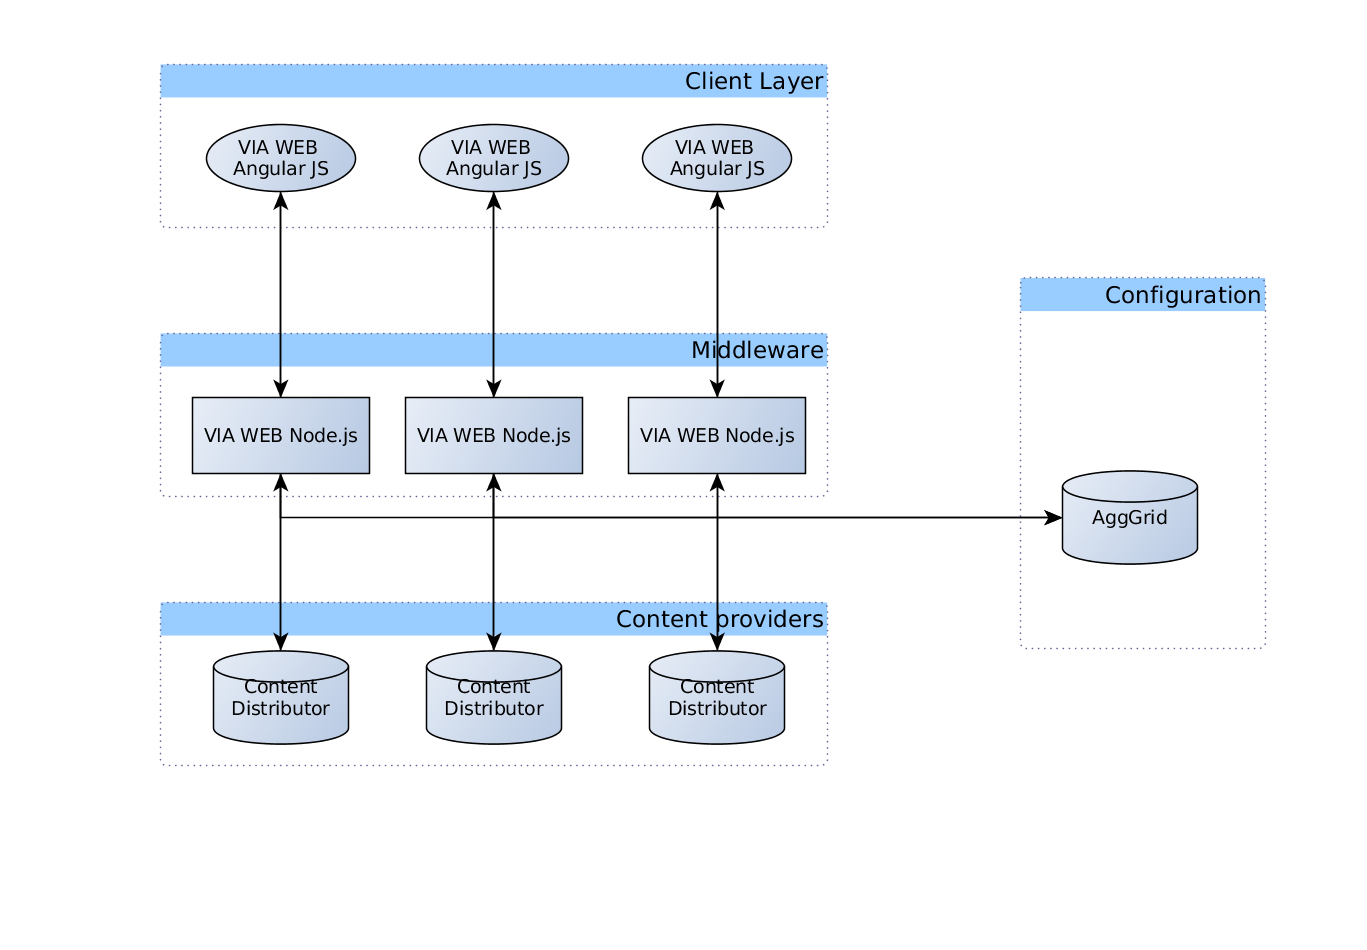
\includegraphics[width=\textwidth]{images/thesis_global_architecture_existing.png}
    \caption{Global architecture overview}
    \label{fig:arch_overview}
\end{figure}


The WEB Angular.js is a web application developed using Javascript, HTML, CSS framework and Model View Controller pattern. In the system, it is indicated as a client application. It communicates with the middleware server through REST services based on HTTP protocol. The client has several components: Controllers, Managers, and Services. 

The contollers validate the user data, invoke corresponding managers, and render data to the view objects represented by HTML pages. The managers are implemented using Facade pattern\cite{DesignPatterns}. They hold and manage services, construct View Model Objects from service responses, and send them back to the controllers. 

The services are the communication layer between the client application and the middleware server. They communicate via REST protocol based on HTTP protocol. This brings flexibility to the architecture and makes components loosely coupled.
% [describe why it is good?]. 

The WEB Node.js is a middleware server. It has several functions:

\begin{itemize}
	\item serves as a data aggregator and security point
	\item translates requests from the client application to the format understandable by the metadata server or content distributors
	\item gathers data from the content distributors
	\item builds data model objects and sends them as JSON entities to the client application.
\end{itemize}

Content servers (content distributors) are customer servers. They are the main sources of information that need to be presented by the client application. They can be represented, for example, by the movie entities or music distributors.

The metadata server is the company-developed server that stores and processes auxiliary and configurational information. The requests can be: 

\begin{itemize}
	\item Data aggregation - required for analytical purposes
	\item User action logs 
	\item User settings - specific user settings, for example, watch history for movie entities
	\item Client and middleware configuration
\end{itemize} 

The interaction between components can be described as follows: the client application initiates the process by sending requests to the middleware server. The middleware server then redirects requests to the underlying servers (content distributors or metadata server), builds data model objects, and sends them to the client application. The client request can be one of two types, configurational or data demand. If the request is configurational, the middleware server redirects it to the metadata server; otherwise, it redirects the request to the content server. The middleware supports the local cache and caches every response that is not associated with the user session. The message diagram between architecture components is depicted on figure \ref{fig:arch_uml}.


\begin{figure}[h]
\begin{center}

	\resizebox{1.0\textwidth}{0.8\textwidth} {

	\begin{sequencediagram}
	\newthread[white]{cl}{Client}
	\newinst[1.7]{mw}{Middleware}
	\newinst{lc}{Local Cache}
	\newinst[1.9]{ms}{Metadata Server}
	\newinst[1.3]{cs}{Content Server}

	\begin{call}{cl}{First request}{mw}{Response}

		\begin{call}{mw}{Create new session}{ms}{Session ID}
		\end{call}

		\begin{call}{mw}{Cache Session}{lc}{}
		\end{call}

		\begin{call}{mw}{Get content locator}{ms}{URL}
		\end{call}

		\begin{call}{mw}{Cache Locator}{lc}{}
		\end{call}

	\end{call}

	\begin{call}{cl}{GET Request}{mw}{GET Response}
		
		\begin{call}{mw}{Check Local Cache}{lc}{}
		\end{call}

		\begin{sdblock}{alt}{if data in cache}
			\begin{call}{mw}{Send response to Client}{cl}{}
			\end{call}
			\begin{sdblock}{else}{}
				\begin{call}{mw}{Request Content}{cs}{Response}
				\end{call}
				\begin{call}{mw}{Cache content}{lc}{}
				\end{call}
			\end{sdblock}
		\end{sdblock}


	\end{call}

	\end{sequencediagram}
	}

\end{center}
\caption{Sequence Diagram of message exchanging}
\label{fig:arch_uml}
\end{figure}

\subsection{Model objects}

In order to understand the existing architecture several definitions should be introduced: Data model object, View Model Object and Application model object.

The data from the content servers differ from one another; as a result, the structure for representing content server objects should be generated dynamically. The asset from the content distributor that has a dynamic structure is called \textit{Data Model Object}(DMO). For example, the DMO can represent information about videos, music, or any other entities. The DMO is generated by the DMO builders from JSON by the middleware server.

The middleware server sends DMOs to the client application. The client application gathers several DMOs and constructs a \textit{View Model Object}(VMO). This object is then presented to the users as a view asset. As a result, the VMO can be defined as a set of data model objects. The VMO is constructed for each HTML page. 

Each content distributor has a set of assets called \textit{Application Model Object}(AMO). Therefore, the application model object is the array of View Model Objects. The AMO represents the information and objects that can be fetched from the single content server.


\subsection{Middleware server architecture}

The middleware server is developed using server side Javascript language and asynchronous server Node.js \cite{Nodejs}. The server is developed using Model View Controller (MVC) pattern and communicates with other components through REST services. As a result, the server components are loosely coupled with each other which gives great flexibility in changing and replacing components and simplifies testing. 

The middleware contains the following components: Controllers, Managers, Services, Configuration and Data Model Object builders. The interraction between components is presented in figure \ref{fig:ms_req}.

\begin{figure}[h]
\begin{center}

	\resizebox{1.0\textwidth}{0.7\textwidth} {

	\begin{sequencediagram}
	\newthread[white]{cl}{Client}
	\newinst[1.7]{cntr}{Controller}
	\newinst[1.3]{mgr}{Manager}
	\newinst[1.3]{lc}{Local Cache}
	\newinst[1.3]{serv}{Service}
	\newinst[1.3]{es}{External Server}

	\begin{call}{cl}{Configuration request}{cntr}{Response}

		\begin{call}{cntr}{Invoke configuation manager}{mgr}{Response Data}
			\begin{call}{mgr}{Check Session key}{lc}{Cache Response}\end{call}
			\begin{sdblock}{alt}{if session key not in cache}
				\begin{call}{mgr}{Get session key using UUID}{serv}{Session key}
					\begin{call}{serv}{Session key request}{es}{Server response}
					\end{call}
				\end{call}
			\end{sdblock}
			\begin{call}{mgr}{Call data service}{serv}{JSON Data}
				\begin{call}{serv}{Call REST API}{es}{JSON data}
				\end{call}
			\end{call}
			\begin{call}{mgr}{Cache response}{lc}{}
			\end{call}
			\begin{call}{mgr}{Make DMO}{mgr}{DMO}\end{call}
		\end{call}

	\end{call}

	\end{sequencediagram}
	}

\end{center}
\caption{Sequence Diagram of Middleware Server Request Process}
\label{fig:ms_req}
\end{figure}

The controllers accept requests from clients. They validate user data and invoke corresponding managers.

The middleware server managers are similar to the client application managers: they implement facade pattern, aggregate multiple services, and redirect requests to them. They also gather the data from services and build immutable Data Model Objects (DMOs). These DMOs are sent back to the client as responses. The workflow of managers is depicted in figure \ref{fig:via_manager}.

\begin{figure}[h]
    \centering
	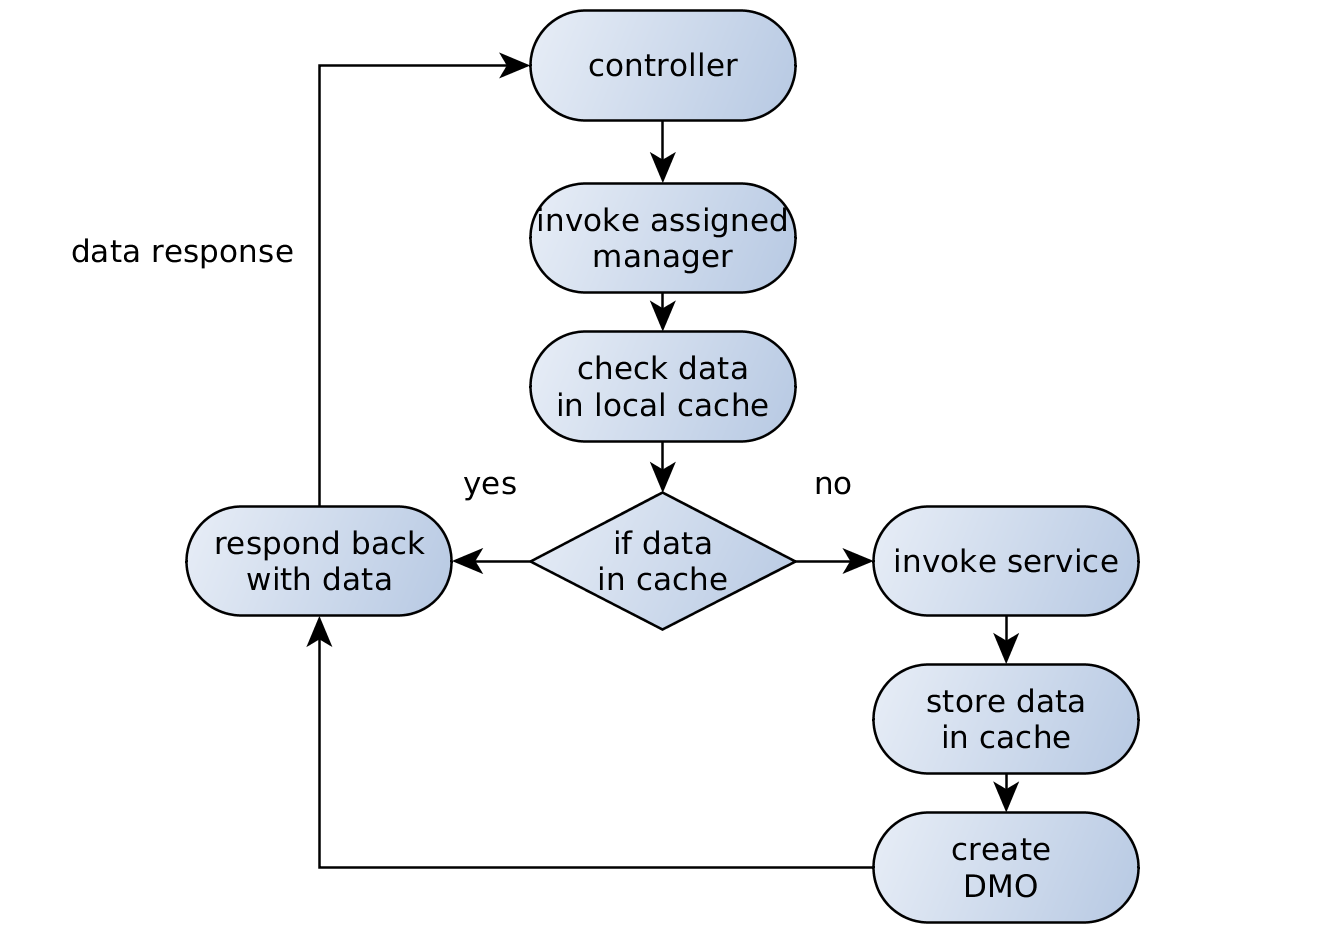
\includegraphics[width=\textwidth]{images/via_manager_1.png}
    \caption{Manager workflow}
    \label{fig:via_manager}
\end{figure}

The middleware services communicate with metadata and content servers. They aggregate the cache layer and react according to the following algorithm: first they check if the data is presented in the local cache; if the service observes cache hit, it will check the object's time to live (TTL) and send the corresponding object back to the manager. On the other hand, if a cache miss occurs, it will send the GET request through the REST protocol to the metadata server or content server, store the response locally for predefined period of time, and send it back to the manager. The workflow of services is presented in figure \ref{fig:via_service}. The time to live is the time (usually specified in seconds) that represents how long the object can be considered fresh without hitting persistence layer.


\begin{figure}[h]
    \centering
	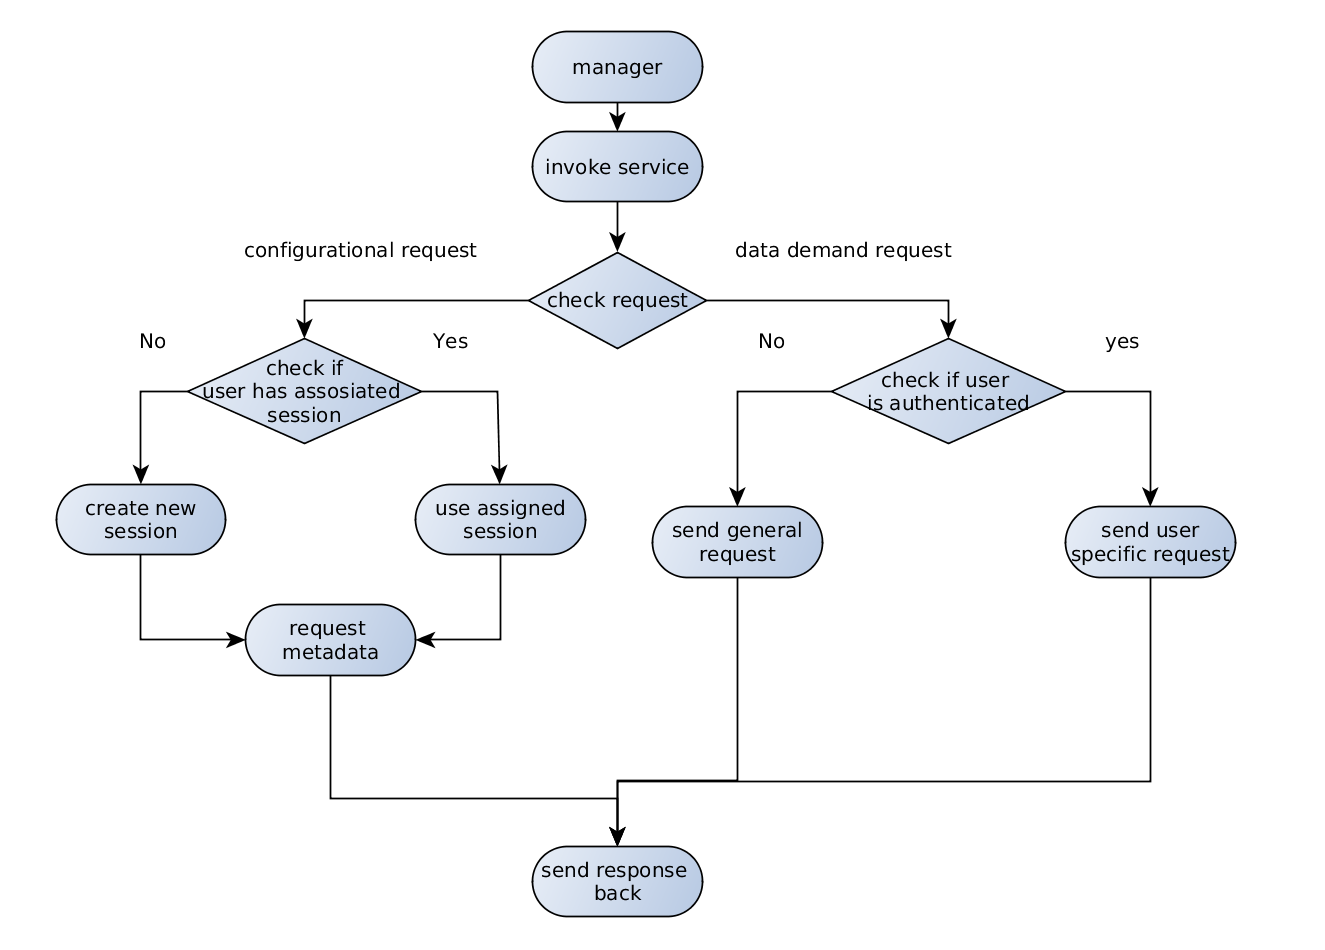
\includegraphics[width=\textwidth]{images/via_service_1.png}
    \caption{Service workflow}
    \label{fig:via_service}
\end{figure}


The client application can make two types of requests: configurational and data demand requests.
The configurational request can have the following purposes:

\begin{itemize}
	\item Provide configuration parameters for both middleware server and client application
	\item Write user activy
	\item Check the health of metadata server
	\item Get Content Server url
	\item User settings and preferences
	\item Analytics
\end{itemize}


The data demand request is a request to the content servers. Since content servers are customer servers, the response doesn't have predefined structure and can have any structure specified by customer service. 

The control flow can be described as follows: the controller receives a request from the client application, validates the data in the request, and redirects it to the assigned manager. The middleware server manager invokes the corresponding service (for example, communications layers). When the client application makes a data demand request, the manager invokes content service that redirects the request to the assigned content server. The response is then stored in the cache, translated into Data Model Object, and transferred back to the client in JSON format. The DMO builders are in charge of translating JSON data into persistent Data Model Objects. For every DMO, there is an assigned manager and service. For example, if the content server responds with a video object, there will be VideoManager and VideoService components.

\subsection{Session management}

The security layer, which is represented by the session management, is responsible for a communication process between the middleware server and inner servers (metadata server and content distributors).

The application session consists of two parts: 

\begin{itemize}
	\item client session
	\item middleware session
\end{itemize}

The purpose of sessions is to distinct between users and provide corresponding analytics to the customers.

The client session is represented by the unique session identifier (UID) and the browser's ID (the string that identifies browser version in the internet). These parameters are generated by the middleware server and transferred to the client through the \textit{set-cookie} header. The browser remembers the data and sends it back with every request in the \textit{cookie} header.


The session is generated per client when he makes the initial request. It contains the metadata session key and the user session, if the user is authenticated. The metadata session is obtained by making a request to the metadata server. The middleware server sends the application key parameter, which is specified in the configuration file and browser ID. The metadata server validates the application key and generates a new session for the middleware server. The middleware server assigns this session to the client and stores it in local memory. The client sends the unique session with each request to the middleware server. The middleware server retrieves the metadata session from the client's request. Using this session, the middleware server can make configurational requests to the metadata server. The sequence diagram of session management is presented in figure \ref{fig:arch_sess_uml}. The application key is given by the system administrator to each middleware server. The browser ID can be any string and does not have validation rules.

\begin{figure}[h]
\begin{center}

	\resizebox{1.1\textwidth}{0.5\textwidth} {

	\begin{sequencediagram}
	\newthread[white]{cl}{Client}
	\newinst[1.5]{md}{Middleware server}
	\newinst[3.0]{mt}{Metadata server}

	\begin{call}{cl}{RequestSession}{md}{Client session}

		\begin{call}{md}{GenerateSessionId}{md}{ClientSessionId} \end{call}
		\begin{call}{md}{GenerateBrowserId}{md}{BrowserId} \end{call}
		\begin{call}{md}{RequestMetadataSession}{mt}{MetadataSession} 
			\begin{call}{mt}{Validate Data}{mt}{}\end{call}
		\end{call}

	\end{call}

	\end{sequencediagram}
	}

\end{center}
\caption{Sequence Diagram of Middleware Session generation}
\label{fig:arch_sess_uml}
\end{figure}


\subsection{Drawbacks of the current architecture}

After careful examination, two categories of problems were defined: client application drawbacks and middleware server drawbacks. 

In order to render the page, the client needs to generate a view model object. The VMO contains several data model objects. The client makes a request for every DMO, aggregates the response, generates VMO from DMOs, and renders it to the HTML view. The drawback is that the client has to make several HTTP requests in order to generate a single VMO. It would be better for the client to make a request for VMO instead of DMO. This approach has some advantages: the client will make less HTTP requests which will increase the performance by reducing the latency and simplify the client's logic considering the client will not be required to generate VMOs from DMOs. 

Another problem with the current client implementation is that it is not generic. If a new content server is introduced, a lot of code would have to be modified on the client side in order to implement the new logic. To solve this, the client can maintain the caching layer that will cache VMOs from the responses. 

Additional complications occur when the client implements MVC pattern, which produces duplication with the middleware server. This approach increases the complexity of the system, since the developers would have to support both the client and the middleware MVC applications. To rectify this, we can simplify the client application and assign two tasks to it: caching and rendering VMOs.

On the middleware side, the DMOs are not generic. The purpose of the middleware server is to serve as a transparent layer, but without dynamic DMO generation a lot of code has to be changed when the new content server is introduced.

The middleware cache can be replaced by the Content Delivery Network (CDN). The middleware caches only information that is common for every user. This work can be done by the CDN edge servers. These will decrease the middleware complexity and decrease the cost of maintaining middleware server.


\newpage

\section{Results}

\subsection{Test Environment}

\subsection{Comparison}

\subsection{Conclusion}

\newpage

\newpage
\section{Discussion and Conclusion}
	
Several conclusions can be made using the results of previous chapter: 

\begin{itemize}
	\item The Hierarchical VMO Generator(HVG) works slower than company's solution without first level cache
	\item The stability of HVG depends on the amount of transferred data: the less data the more stable responses
	\item Without latency (that was introduced artificially) the HVG with optimal configuration works roughly with the same speed as current company solution where VMOs are generated on the client side
	\item With latency the HVG solution works faster 
\end{itemize}

The \cite{VarnApacheReverse} gives the detailed evaluation of Apache Traffic server and Varnish server; As a result, the comparison between them is omitted in this project. 

The HVG solution consumes more CPU and memory because it stores the graph of data model objects plus the fetched data from content distributors. It uses computationally intensive breadth first search algorithm on directed graph. On the other hand, the client side VMO generation sends multiple simple requests to the middleware server. They are light requests, that consume small amount of CPU power and memory and is used just for storing the final dta model object.

Fortunately, the algorithm for generating HVG is executed rarely because most of the time the data is retrieved in the VMO cache. The drawback of this approach is that the data is stored two times: one as a part of Data Model Object, another as a part of View Model Object. The Data Model Object cache could be turned off, unfortunately these will give additional problems: if the VMO will be stored for the time equals of maximum TTL among all DMOs, some DMOs will become stale and the server response will be irrelevant. Taking this in consideration, the maximum TTL for VMO is computed as:

\begin{center}
	\begin{math}M = \min_{1 \leq i \leq N} D_{i},\{i=1:N\}\end{math}, N - amount of DMOs that need to be fetched in request.
\end{center}

Theoretically, the solution with HVG does not work well when the set of DMOs have TTL that dramatically differs from one another. In this case, the overhead produced by VMO computation will be greater than the latency for retrieving data model objects, but in general it requires additional study. 

\subsection{Further studies}

The Application Model Object(AMO) should be studied and corresponding conclusions should be produced. For small VMOs, perhaps it would be more optimal to transfer compressed AMO.

The Web cache solution requires additional study in terms of selecting the appropriate algorithm for calculating TTL (time to live) of VMO/DMO objects. Currently the TTL is set to the default time that was not selected through careful study. The maximum time for VMO equals the TTL of DMO that has minumum value. This is one of the proposed algorithms, however this question is not studied enough and requires futher work.

\newpage

\begin{thebibliography}{99}

% \bibitem{norvig06}
%   П. Норвиг, С. Рассел,
%   \emph{Искусственный интеллект: современный подход}, 2-е изд.
%   М.: Издательский дом ``Вильямс'',
%   2006.

% \bibitem{forsight04}
%   Д. Форсайт, Ж. Понс,
%   \emph{Компьютерное зрение. Современный подход}.
%   М.: Издательский дом ``Вильямс'',
%   2004.

\end{thebibliography}


\end{document}
